% Copyright (C) 2021 Erwin Müller <erwin@muellerpublic.de>
% Released as open-source under the Apache License, Version 2.0.
%
% ****************************************************************************
% ANL-OpenCL :: Docs
% ****************************************************************************
%
% Copyright (C) 2021 Erwin Müller <erwin@muellerpublic.de>
%
% Licensed under the Apache License, Version 2.0 (the "License");
% you may not use this file except in compliance with the License.
% You may obtain a copy of the License at
%
%      http://www.apache.org/licenses/LICENSE-2.0
%
% Unless required by applicable law or agreed to in writing, software
% distributed under the License is distributed on an "AS IS" BASIS,
% WITHOUT WARRANTIES OR CONDITIONS OF ANY KIND, either express or implied.
% See the License for the specific language governing permissions and
% limitations under the License.
%
% ****************************************************************************
% ANL-OpenCL :: Docs is a derivative work based on Josua Tippetts' C++ library:
% http://accidentalnoise.sourceforge.net/index.html
% ****************************************************************************
%
% Copyright (C) 2011 Joshua Tippetts
%
%   This software is provided 'as-is', without any express or implied
%   warranty.  In no event will the authors be held liable for any damages
%   arising from the use of this software.
%
%   Permission is granted to anyone to use this software for any purpose,
%   including commercial applications, and to alter it and redistribute it
%   freely, subject to the following restrictions:
%
%   1. The origin of this software must not be misrepresented; you must not
%      claim that you wrote the original software. If you use this software
%      in a product, an acknowledgment in the product documentation would be
%      appreciated but is not required.
%   2. Altered source versions must be plainly marked as such, and must not be
%      misrepresented as being the original software.
%   3. This notice may not be removed or altered from any source distribution.
%
%
% ****************************************************************************
% ANL-OpenCL :: Docs bundles and uses the RandomCL library:
% https://github.com/bstatcomp/RandomCL
% ****************************************************************************
%
% BSD 3-Clause License
%
% Copyright (c) 2018, Tadej Ciglarič, Erik Štrumbelj, Rok Češnovar. All rights reserved.
%
% Redistribution and use in source and binary forms, with or without modification, are permitted provided that the following conditions are met:
%
% * Redistributions of source code must retain the above copyright notice, this list of conditions and the following disclaimer.
%
% * Redistributions in binary form must reproduce the above copyright notice, this list of conditions and the following disclaimer in the documentation and/or other materials provided with the distribution.
%
% * Neither the name of the copyright holder nor the names of its contributors may be used to endorse or promote products derived from this software without specific prior written permission.
%
% THIS SOFTWARE IS PROVIDED BY THE COPYRIGHT HOLDERS AND CONTRIBUTORS "AS IS" AND ANY EXPRESS OR IMPLIED WARRANTIES, INCLUDING, BUT NOT LIMITED TO, THE IMPLIED WARRANTIES OF MERCHANTABILITY AND FITNESS FOR A PARTICULAR PURPOSE ARE DISCLAIMED. IN NO EVENT SHALL THE COPYRIGHT HOLDER OR CONTRIBUTORS BE LIABLE FOR ANY DIRECT, INDIRECT, INCIDENTAL, SPECIAL, EXEMPLARY, OR CONSEQUENTIAL DAMAGES (INCLUDING, BUT NOT LIMITED TO, PROCUREMENT OF SUBSTITUTE GOODS OR SERVICES; LOSS OF USE, DATA, OR PROFITS; OR BUSINESS INTERRUPTION) HOWEVER CAUSED AND ON ANY THEORY OF LIABILITY, WHETHER IN CONTRACT, STRICT LIABILITY, OR TORT (INCLUDING NEGLIGENCE OR OTHERWISE) ARISING IN ANY WAY OUT OF THE USE OF THIS SOFTWARE, EVEN IF ADVISED OF THE POSSIBILITY OF SUCH DAMAGE.

\subsection{Kernel Functions}

Since \ANLOpenCL/ is a port of the Josua Tippetts' C++ library
\url{http://accidentalnoise.sourceforge.net/index.html} the same documentation
can be used for the noise generation functions.
All of the functions and types are defined in the \ANLOpenCLTypeIndex{kernel.h}.

\subsubsection{Manipulation Functions}

\index{rotateDomain3}\index{rotateDomain4}\index{rotateDomain6}
\begin{lstlisting}[caption={Definition of rotate domain functions},label={lst:rotate_domain_definition},language=OpenCL]
vector3 rotateDomain3(vector3 src, REAL angle, REAL ax, REAL ay, REAL az);
vector4 rotateDomain4(vector4 src, REAL angle, REAL ax, REAL ay, REAL az);
vector8 rotateDomain6(vector8 src, REAL angle, REAL ax, REAL ay, REAL az);
\end{lstlisting}

\begin{lstlisting}[caption={Example for rotate domain functions},label={lst:rotate_domain_example},language=OpenCL]
kernel void map2d_image(
global struct SMappingRanges *g_ranges,
write_only image2d_t output
) {
    $insert_localMapRange
    long seed = 200;
    vector3 rotated = rotateDomain3(coord[i], radians(90), 1, 0, 0);
    const float v = value_noise3D(rotated, seed, linearInterp);
    write_imagef(output, (int2)(g0, g1), (float4)(v, v, v, 1.0));
}
\end{lstlisting}

Rotates the source coordinates by the angle over the rotation axis.

\index{scaleDomain}
\begin{lstlisting}[caption={Definition of scale domain function},label={lst:scale_domain_definition},language=OpenCL]
scaleDomain(v, scale)
\end{lstlisting}

\begin{lstlisting}[caption={Example for scale domain function},label={lst:scale_domain_example},language=OpenCL]
kernel void map2d_image(
global struct SMappingRanges *g_ranges,
write_only image2d_t output
) {
    $insert_localMapRange
    long seed = 200;
    vector3 scaled = scaleDomain(coord[i], 10);
    const float v = value_noise3D(scaled, seed, linearInterp);
    write_imagef(output, (int2)(g0, g1), (float4)(v, v, v, 1.0));
}
\end{lstlisting}

Multiplies the source coordinates by the scale.

\index{combineRGBA}\index{combineHSVA}
\begin{lstlisting}[caption={Definition of combine color values functions},label={lst:combine_color_definition},language=OpenCL]
vector4 combineRGBA(REAL r, REAL g, REAL b, REAL a);
vector4 combineHSVA(REAL h, REAL s, REAL v, REAL a);
\end{lstlisting}

\begin{lstlisting}[caption={Example for scale domain function},label={lst:combine_color_example},language=OpenCL]
kernel void map2d_image(
global struct SMappingRanges *g_ranges,
write_only image2d_t output
) {
    $insert_localMapRange
    long seed = 200;
    const float r = value_noise3D(coord[i], seed, linearInterp);
    const float g = value_noise3D(coord[i], seed*10, linearInterp);
    const float b = value_noise3D(coord[i], seed*100, linearInterp);
    const vector4 c = combineRGBA(r, g, b, 1.0);
    write_imagef(output, (int2)(g0, g1), c);
}
\end{lstlisting}

Combines the RGBA or HSVA values.

\subsubsection{Fractal Layer Functions}

\begin{figure}[h]
\centering
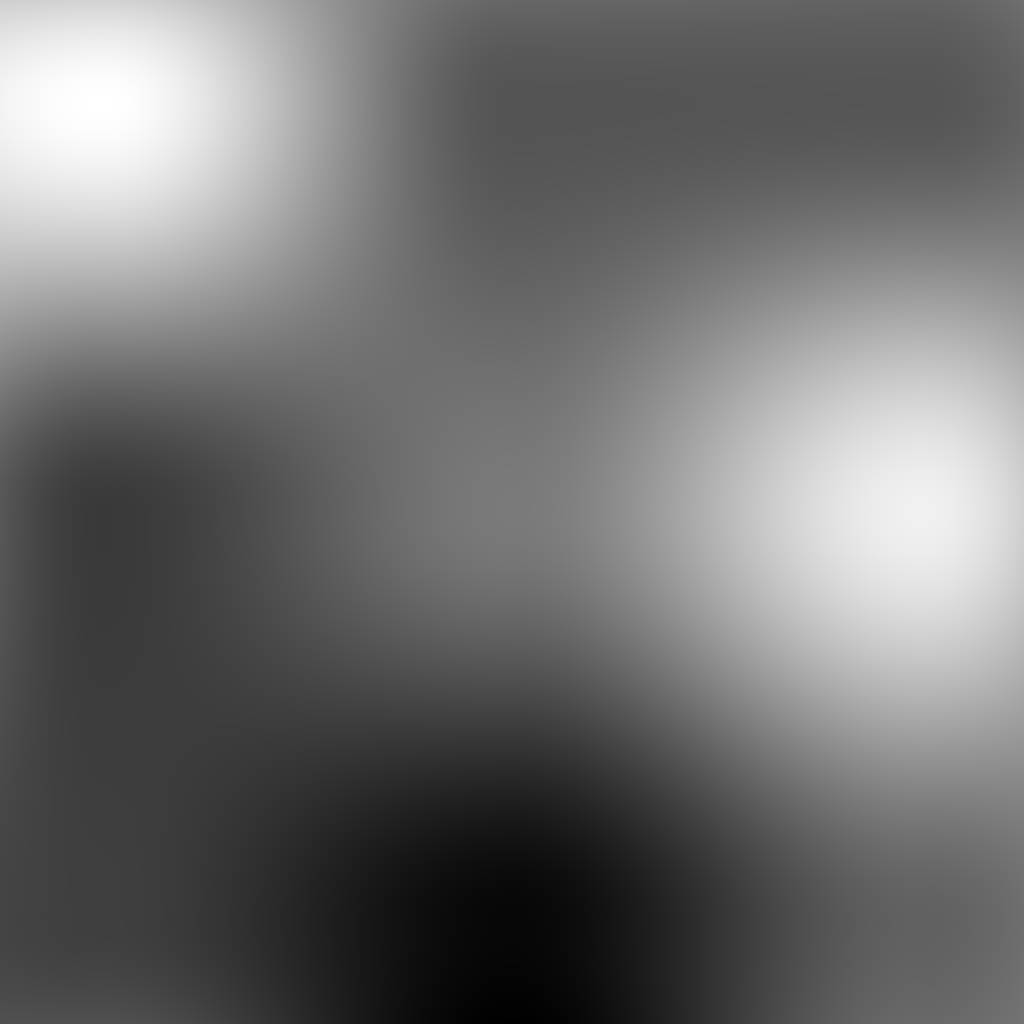
\includegraphics[width=0.4\textwidth]{out/simpleFractalLayer3/simpleFractalLayer3_value_noise3D_hermiteInterp_rot.png}
\caption{Simple fractal layer with value noise 3D and hermite interpolation with rotation.}
\label{fig:simple_fractal_layer3_value_noise3D_hermiteInterp_rot}
\end{figure}

\begin{figure}[h]
\centering
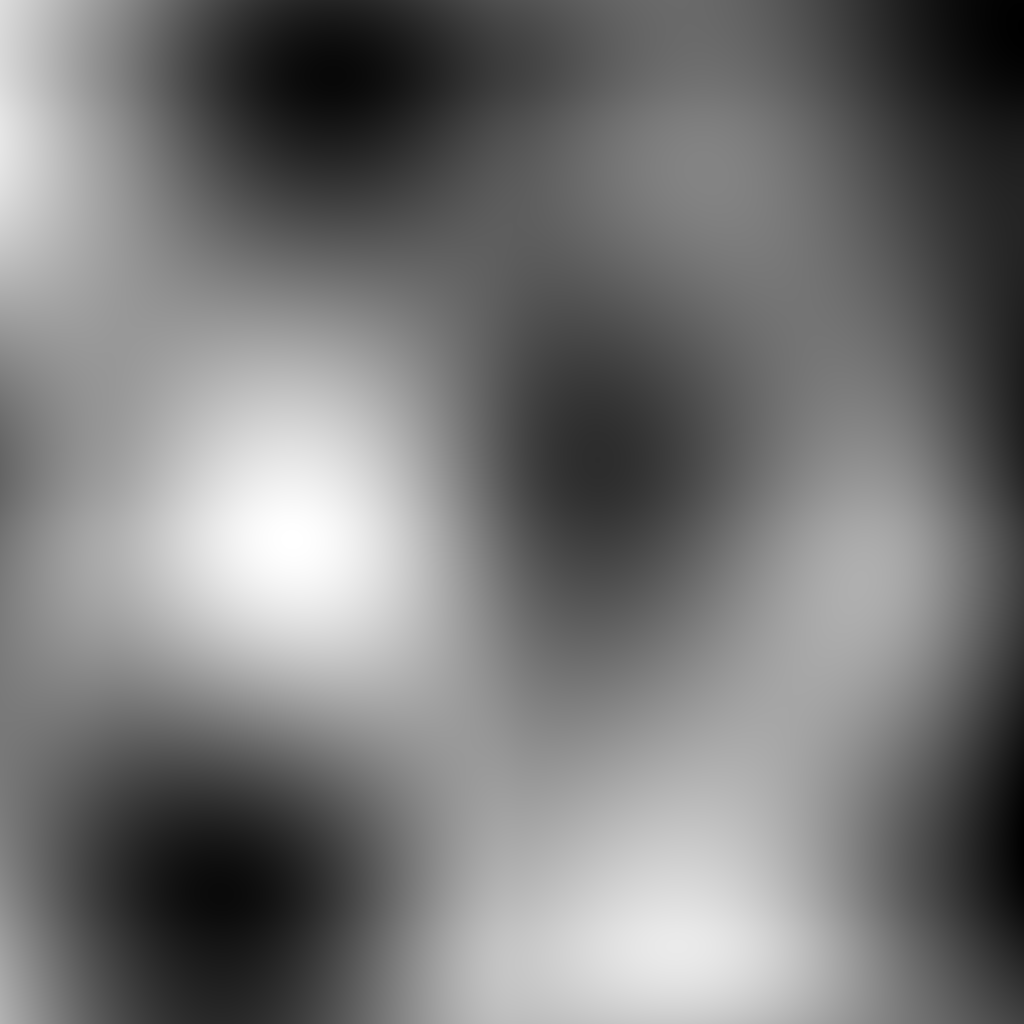
\includegraphics[width=0.4\textwidth]{out/simpleFractalLayer3/simpleFractalLayer3_gradient_noise3D_hermiteInterp_rot.png}
\caption{Simple fractal layer with gradient noise 3D and linear hermite with rotation.}
\label{fig:simple_fractal_layer3_gradient_noise3D_hermiteInterp_rot}
\end{figure}

\begin{figure}[h]
\centering
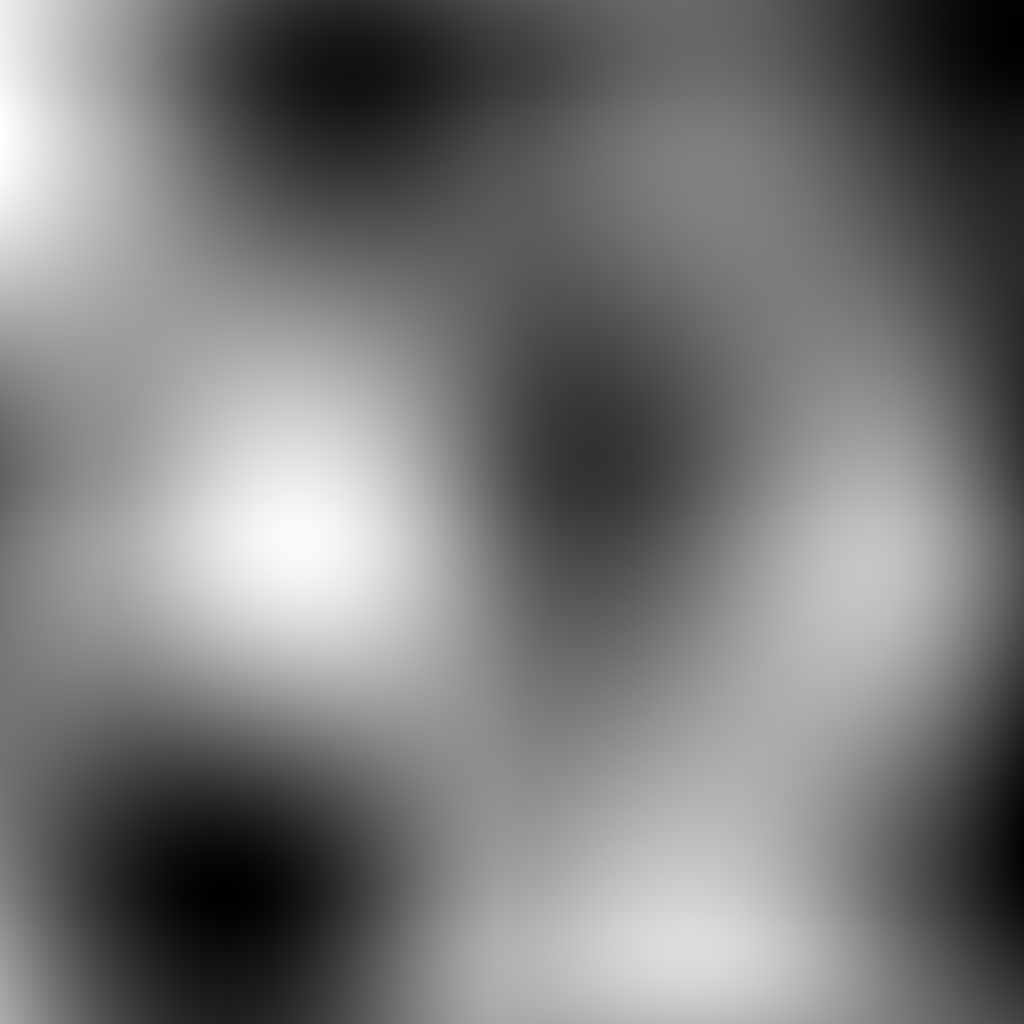
\includegraphics[width=0.4\textwidth]{out/simpleFractalLayer3/simpleFractalLayer3_gradval_noise3D_hermiteInterp_rot.png}
\caption{Simple fractal layer with gradval noise 3D and hermite interpolation with rotation.}
\label{fig:simple_fractal_layer3_gradval_noise3D_hermiteInterp_rot}
\end{figure}

\begin{figure}[h]
\centering
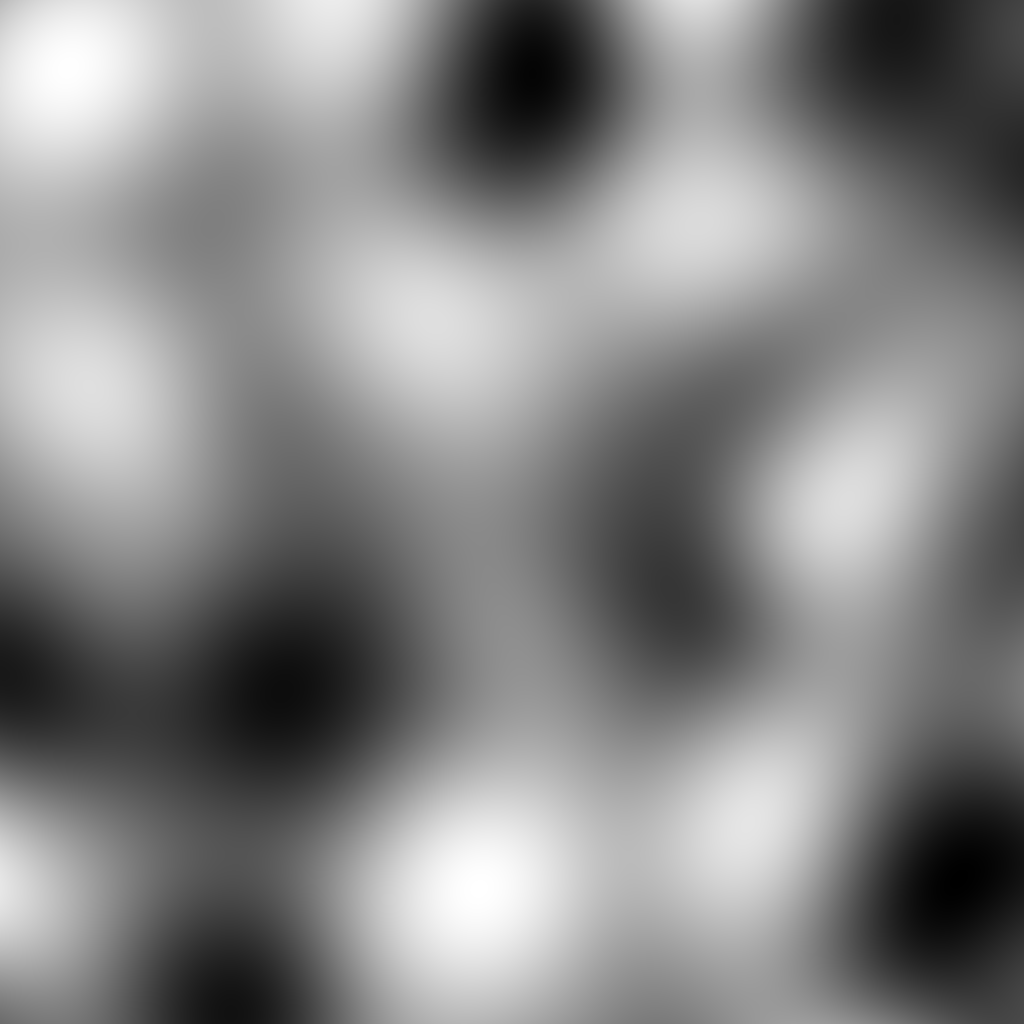
\includegraphics[width=0.4\textwidth]{out/simpleFractalLayer3/simpleFractalLayer3_simplex_noise3D_noInterp_rot.png}
\caption{Simple fractal layer with simplex noise 3D with rotation.}
\label{fig:simple_fractal_layer3_simplex_noise3D_noInterp_rot}
\end{figure}

\index{simpleFractalLayer3}\index{simpleFractalLayer4}\index{simpleFractalLayer6}
\begin{lstlisting}[caption={Definition of simple fractal layer functions},label={lst:simple_fractal_layer_definition},language=OpenCL]
REAL simpleFractalLayer3(vector3 v, noise_func3 basistype, uint seed, interp_func interp, REAL layerscale, REAL layerfreq, bool rot, REAL angle, REAL ax, REAL ay, REAL az);
REAL simpleFractalLayer4(vector4 v, noise_func4 basistype, uint seed, interp_func interp, REAL layerscale, REAL layerfreq, bool rot, REAL angle, REAL ax, REAL ay, REAL az);
REAL simpleFractalLayer6(vector8 v, noise_func6 basistype, uint seed, interp_func interp, REAL layerscale, REAL layerfreq, bool rot, REAL angle, REAL ax, REAL ay, REAL az);
\end{lstlisting}

\begin{lstlisting}[caption={Example for simple fractal layer functions},label={lst:simple_fractal_layer_example},language=OpenCL]
kernel void map2d_image(
global struct SMappingRanges *g_ranges,
write_only image2d_t output
) {
    $insert_localMapRange
    long seed = 200;
    // no rotation
    const float v = simpleFractalLayer3(coord[i], value_noise3D, 200, noInterp, 1, 0.125, false, 0.0, 0.0, 0.0, 0.0);
    // with rotation
    const float v = simpleFractalLayer3(coord[i], value_noise3D, 200, noInterp, 1, 0.125, true, 1.57, 1.0, 0.0, 0.0);
    write_imagef(output, (int2)(g0, g1), (float4)(v, v, v, 1.0));
}
\end{lstlisting}

Returns simple fractal layer value for the coordinate.

\begin{figure}[h]
\centering

\includegraphics[width=0.4\textwidth]{out/simpleRidgedLayer3/simpleRidgedLayer3_value_noise3D_hermiteInterp_rot.png}
\caption{Ridged fractal layer with value noise 3D and hermite interpolation with rotation.}
\label{fig:ridged_fractal_layer3_value_noise3D_hermiteInterp_rot}
\end{figure}

\begin{figure}[h]
\centering
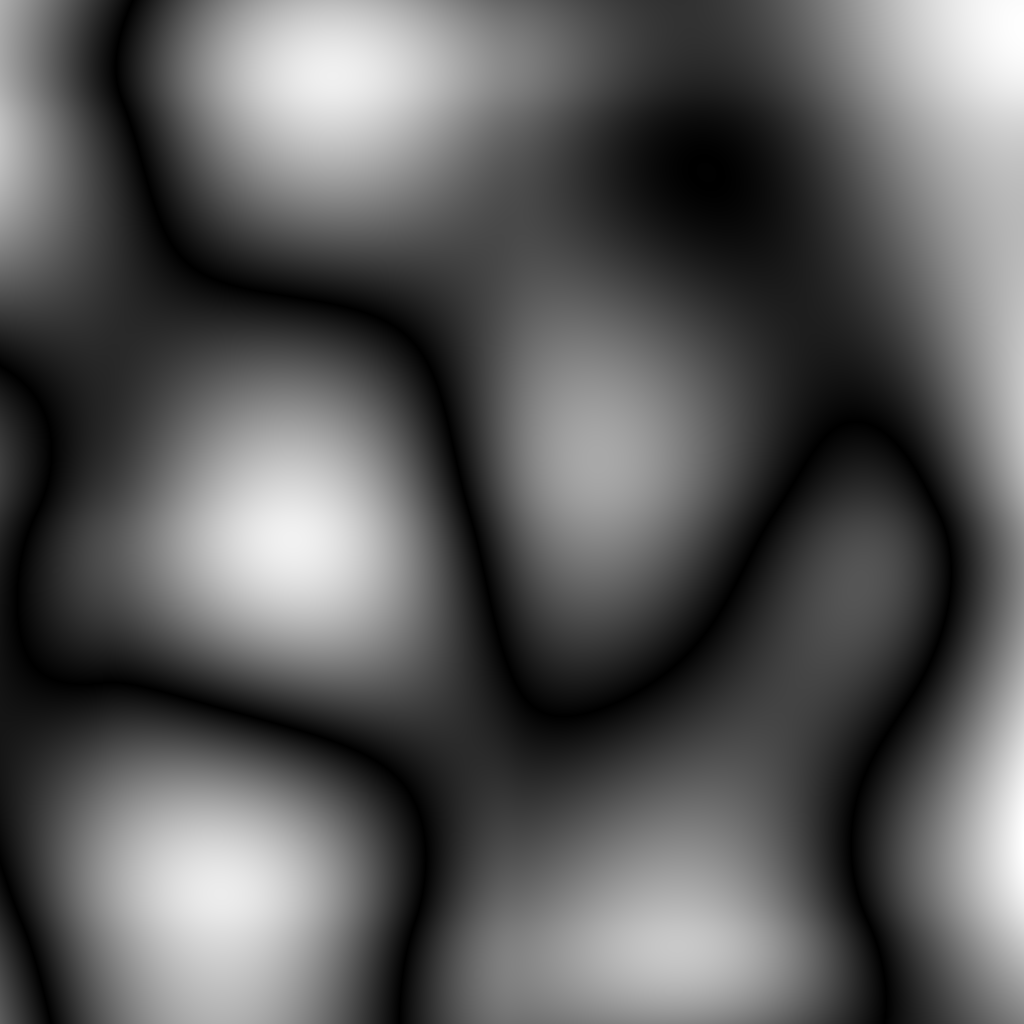
\includegraphics[width=0.4\textwidth]{out/simpleRidgedLayer3/simpleRidgedLayer3_gradient_noise3D_hermiteInterp_rot.png}
\caption{Ridged fractal layer with gradient noise 3D and linear hermite with rotation.}
\label{fig:ridged_fractal_layer3_gradient_noise3D_hermiteInterp_rot}
\end{figure}

\begin{figure}[h]
\centering
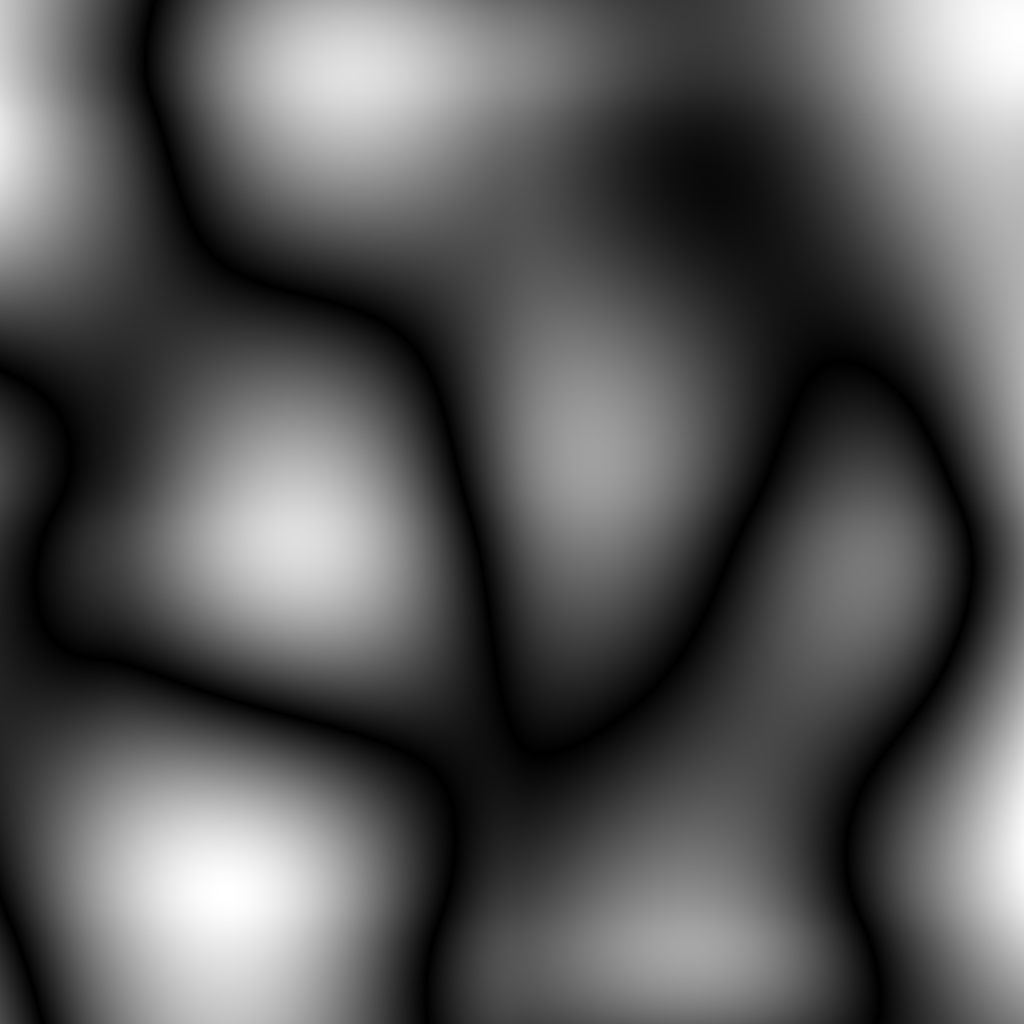
\includegraphics[width=0.4\textwidth]{out/simpleRidgedLayer3/simpleRidgedLayer3_gradval_noise3D_hermiteInterp_rot.png}
\caption{Ridged fractal layer with gradval noise 3D and hermite interpolation with rotation.}
\label{fig:ridged_fractal_layer3_gradval_noise3D_hermiteInterp_rot}
\end{figure}

\begin{figure}[h]
\centering
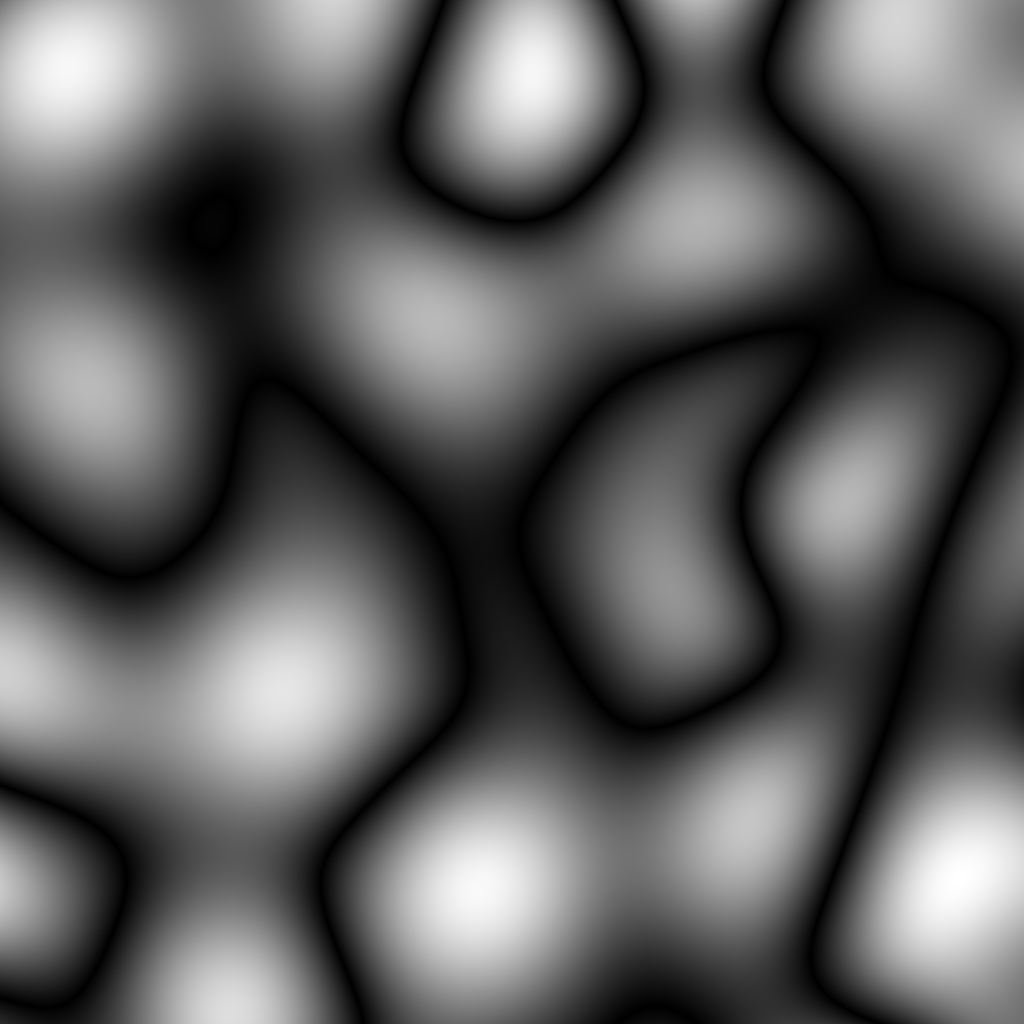
\includegraphics[width=0.4\textwidth]{out/simpleRidgedLayer3/simpleRidgedLayer3_simplex_noise3D_noInterp_rot.png}
\caption{Ridged fractal layer with simplex noise 3D with rotation.}
\label{fig:ridged_fractal_layer3_simplex_noise3D_noInterp_rot}
\end{figure}

\index{simpleRidgedLayer3}\index{simpleRidgedLayer4}\index{simpleRidgedLayer6}
\begin{lstlisting}[caption={Definition of ridged fractal layer functions},label={lst:ridged_fractal_layer_definition},language=OpenCL]
REAL simpleRidgedLayer3(vector3 v, noise_func3 basistype, uint seed, interp_func interp, REAL layerscale, REAL layerfreq, bool rot, REAL angle, REAL ax, REAL ay, REAL az);
REAL simpleRidgedLayer4(vector4 v, noise_func4 basistype, uint seed, interp_func interp, REAL layerscale, REAL layerfreq, bool rot, REAL angle, REAL ax, REAL ay, REAL az);
REAL simpleRidgedLayer6(vector8 v, noise_func6 basistype, uint seed, interp_func interp, REAL layerscale, REAL layerfreq, bool rot, REAL angle, REAL ax, REAL ay, REAL az);
\end{lstlisting}

\begin{lstlisting}[caption={Example for ridged fractal layer functions},label={lst:ridged_fractal_layer_example},language=OpenCL]
kernel void map2d_image(
global struct SMappingRanges *g_ranges,
write_only image2d_t output
) {
    $insert_localMapRange
    long seed = 200;
    // no rotation
    const float v = simpleRidgedLayer3(coord[i], value_noise3D, 200, noInterp, 1, 0.125, false, 0.0, 0.0, 0.0, 0.0);
    // with rotation
    const float v = simpleRidgedLayer3(coord[i], value_noise3D, 200, noInterp, 1, 0.125, true, 1.57, 1.0, 0.0, 0.0);
    write_imagef(output, (int2)(g0, g1), (float4)(v, v, v, 1.0));
}
\end{lstlisting}

Returns simple ridged layer value for the coordinate.

\begin{figure}[h]
\centering

\includegraphics[width=0.4\textwidth]{out/simpleBillowLayer3/simpleBillowLayer3_value_noise3D_hermiteInterp_rot.png}
\caption{Billow fractal layer with value noise 3D and hermite interpolation with rotation.}
\label{fig:billow_fractal_layer3_value_noise3D_hermiteInterp_rot}
\end{figure}

\begin{figure}[h]
\centering
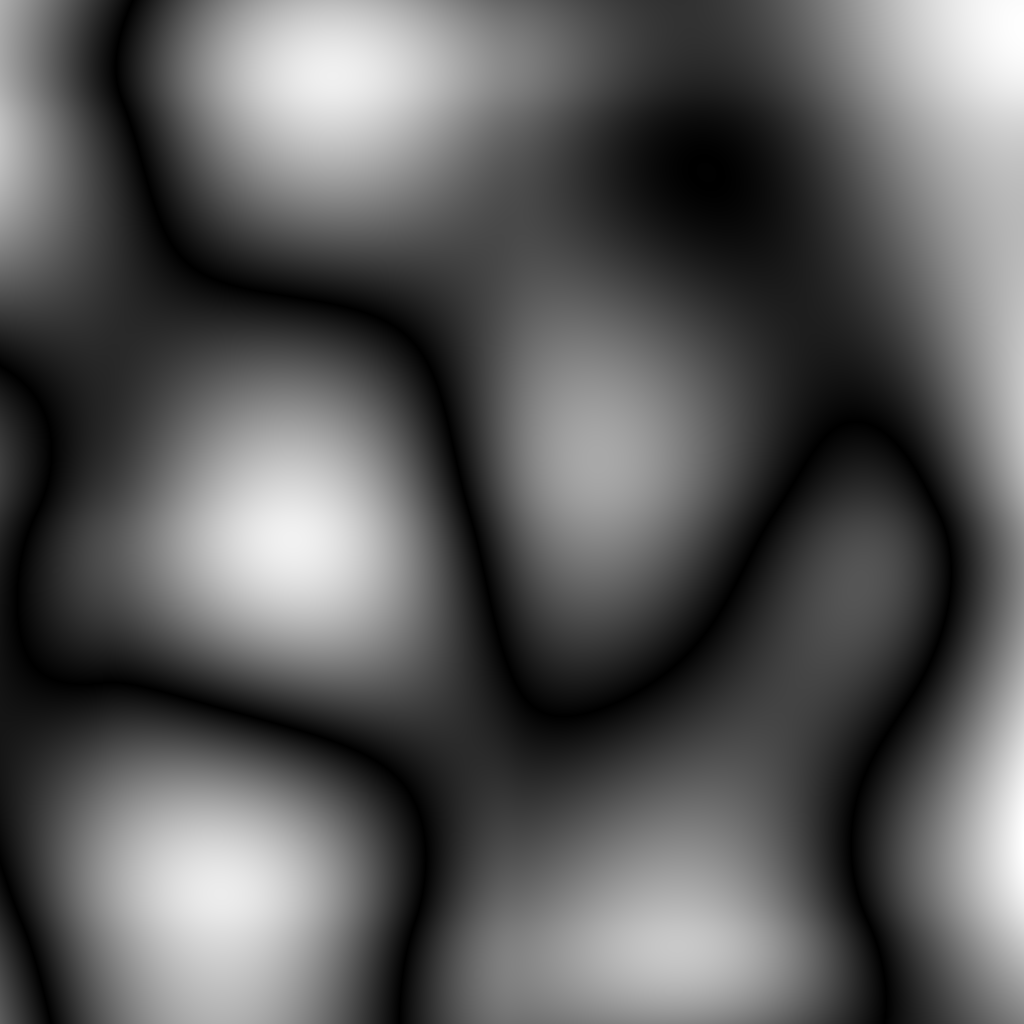
\includegraphics[width=0.4\textwidth]{out/simpleBillowLayer3/simpleBillowLayer3_gradient_noise3D_hermiteInterp_rot.png}
\caption{Billow fractal layer with gradient noise 3D and linear hermite with rotation.}
\label{fig:billow_fractal_layer3_gradient_noise3D_hermiteInterp_rot}
\end{figure}

\begin{figure}[h]
\centering
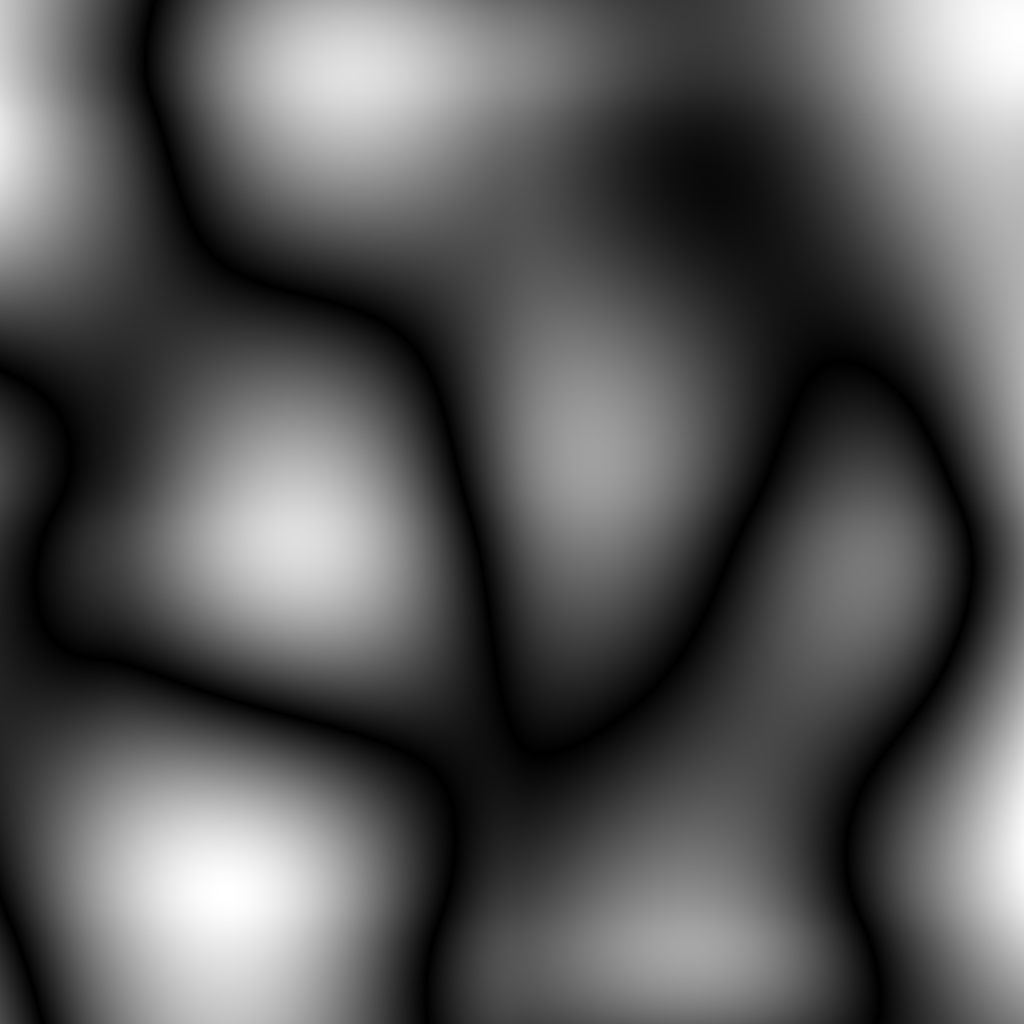
\includegraphics[width=0.4\textwidth]{out/simpleBillowLayer3/simpleBillowLayer3_gradval_noise3D_hermiteInterp_rot.png}
\caption{Billow fractal layer with gradval noise 3D and hermite interpolation with rotation.}
\label{fig:billow_fractal_layer3_gradval_noise3D_hermiteInterp_rot}
\end{figure}

\begin{figure}[h]
\centering
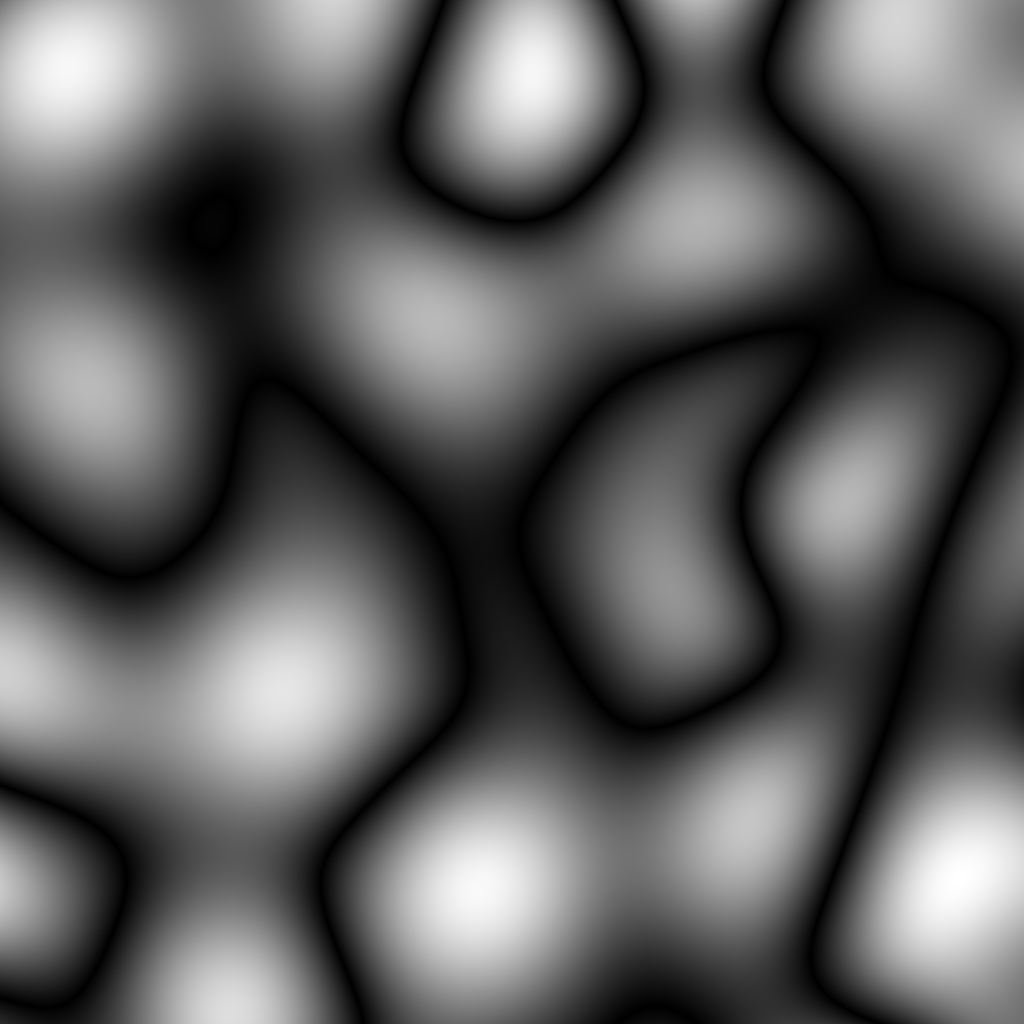
\includegraphics[width=0.4\textwidth]{out/simpleBillowLayer3/simpleBillowLayer3_simplex_noise3D_noInterp_rot.png}
\caption{Billow fractal layer with simplex noise 3D with rotation.}
\label{fig:billow_fractal_layer3_simplex_noise3D_noInterp_rot}
\end{figure}

\index{simpleBillowLayer3}\index{simpleBillowLayer4}\index{simpleBillowLayer6}
\begin{lstlisting}[caption={Definition of billow fractal layer functions},label={lst:billow_fractal_layer_definition},language=OpenCL]
REAL simpleBillowLayer3(vector3 v, noise_func3 basistype, uint seed, interp_func interp, REAL layerscale, REAL layerfreq, bool rot, REAL angle, REAL ax, REAL ay, REAL az);
REAL simpleBillowLayer4(vector4 v, noise_func4 basistype, uint seed, interp_func interp, REAL layerscale, REAL layerfreq, bool rot, REAL angle, REAL ax, REAL ay, REAL az);
REAL simpleBillowLayer6(vector8 v, noise_func6 basistype, uint seed, interp_func interp, REAL layerscale, REAL layerfreq, bool rot, REAL angle, REAL ax, REAL ay, REAL az);
\end{lstlisting}

\begin{lstlisting}[caption={Example for billow fractal layer functions},label={lst:billow_fractal_layer_example},language=OpenCL]
kernel void map2d_image(
global struct SMappingRanges *g_ranges,
write_only image2d_t output
) {
    $insert_localMapRange
    long seed = 200;
    // no rotation
    const float v = simpleBillowLayer3(coord[i], value_noise3D, 200, noInterp, 1, 0.125, false, 0.0, 0.0, 0.0, 0.0);
    // with rotation
    const float v = simpleBillowLayer3(coord[i], value_noise3D, 200, noInterp, 1, 0.125, true, 1.57, 1.0, 0.0, 0.0);
    write_imagef(output, (int2)(g0, g1), (float4)(v, v, v, 1.0));
}
\end{lstlisting}

Returns simple billow layer value for the coordinate.

\subsubsection{Fractal Functions}

\begin{figure}[h]
\centering
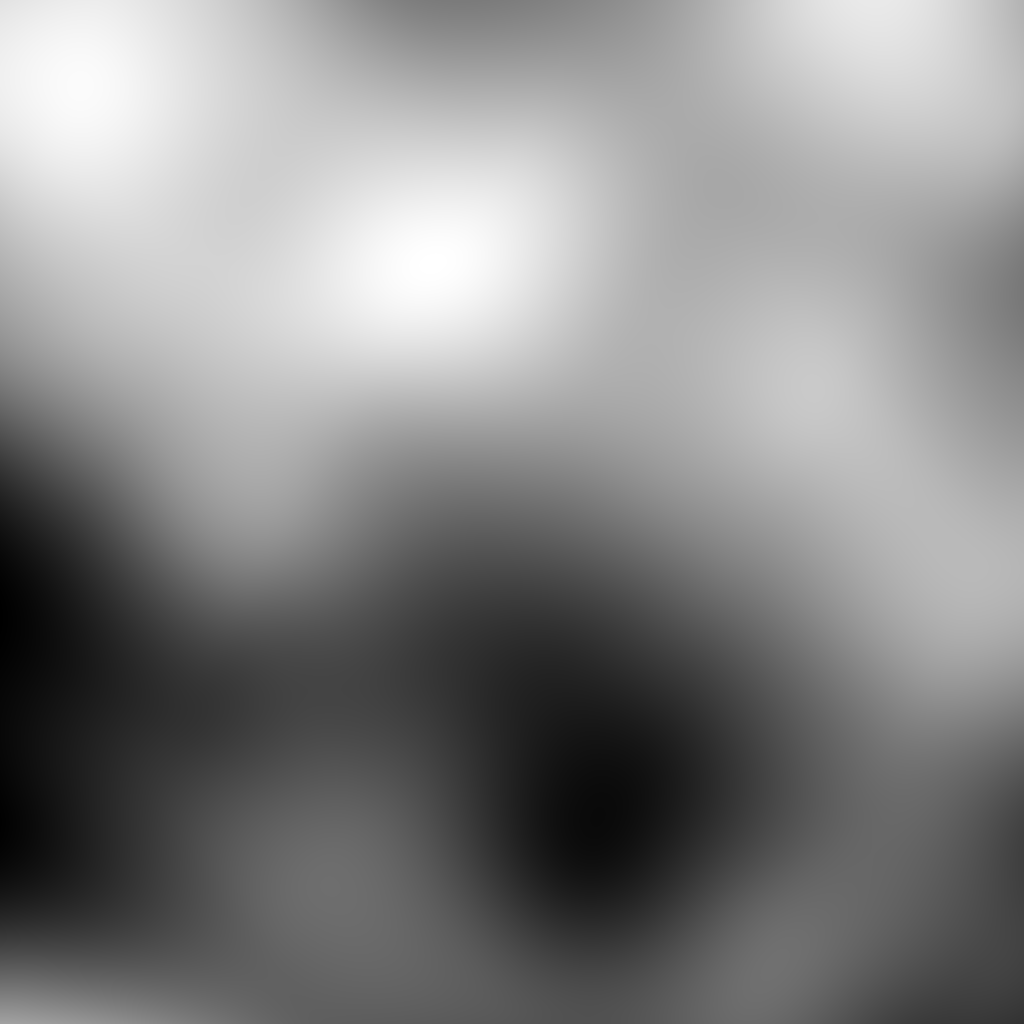
\includegraphics[width=0.4\textwidth]{out/simplefBm3/simplefBm3_value_noise3D_hermiteInterp_rot.png}
\caption{Simple brownian motion fractal with value noise 3D and hermite interpolation with rotation.}
\label{fig:simple_bm3_value_noise3D_hermiteInterp_rot}
\end{figure}

\begin{figure}[h]
\centering
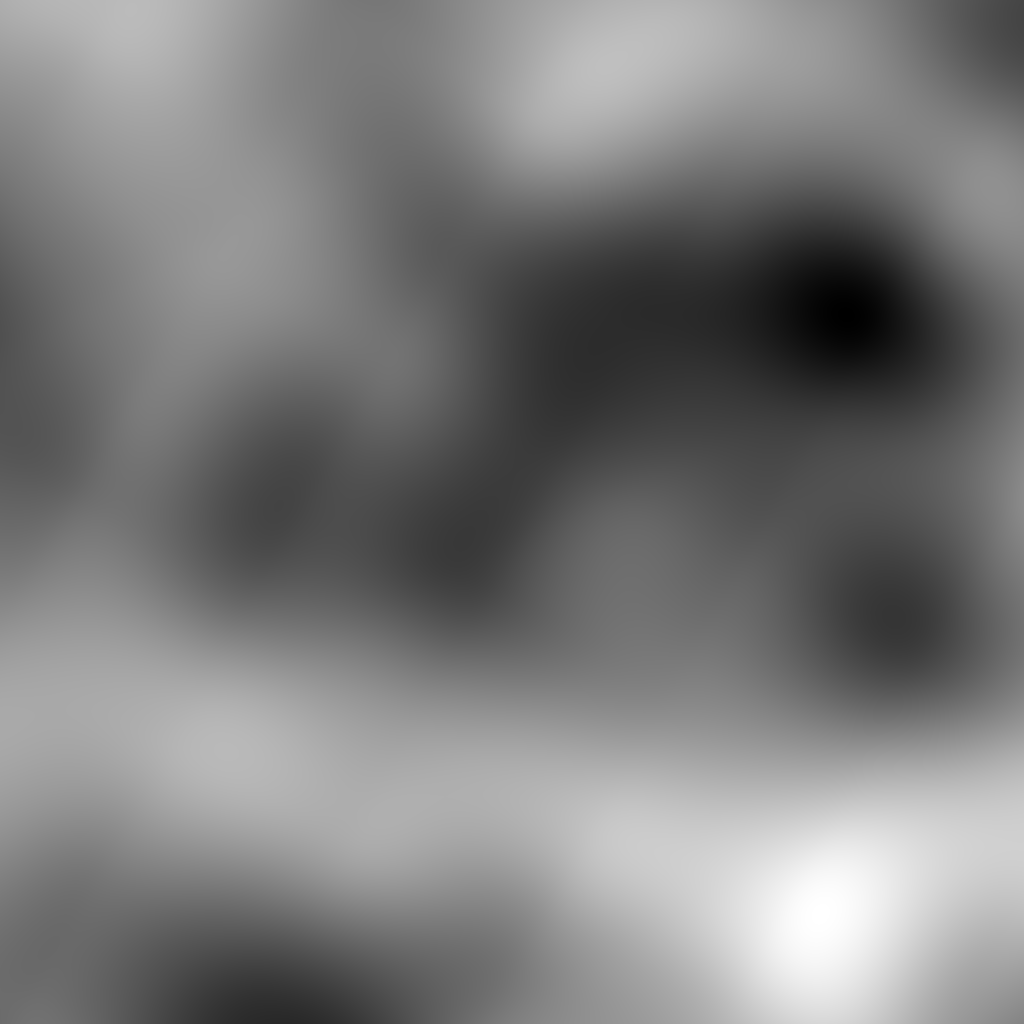
\includegraphics[width=0.4\textwidth]{out/simplefBm3/simplefBm3_gradient_noise3D_hermiteInterp_rot.png}
\caption{Simple brownian motion fractal with gradient noise 3D and linear hermite with rotation.}
\label{fig:simple_bm3_gradient_noise3D_hermiteInterp_rot}
\end{figure}

\begin{figure}[h]
\centering
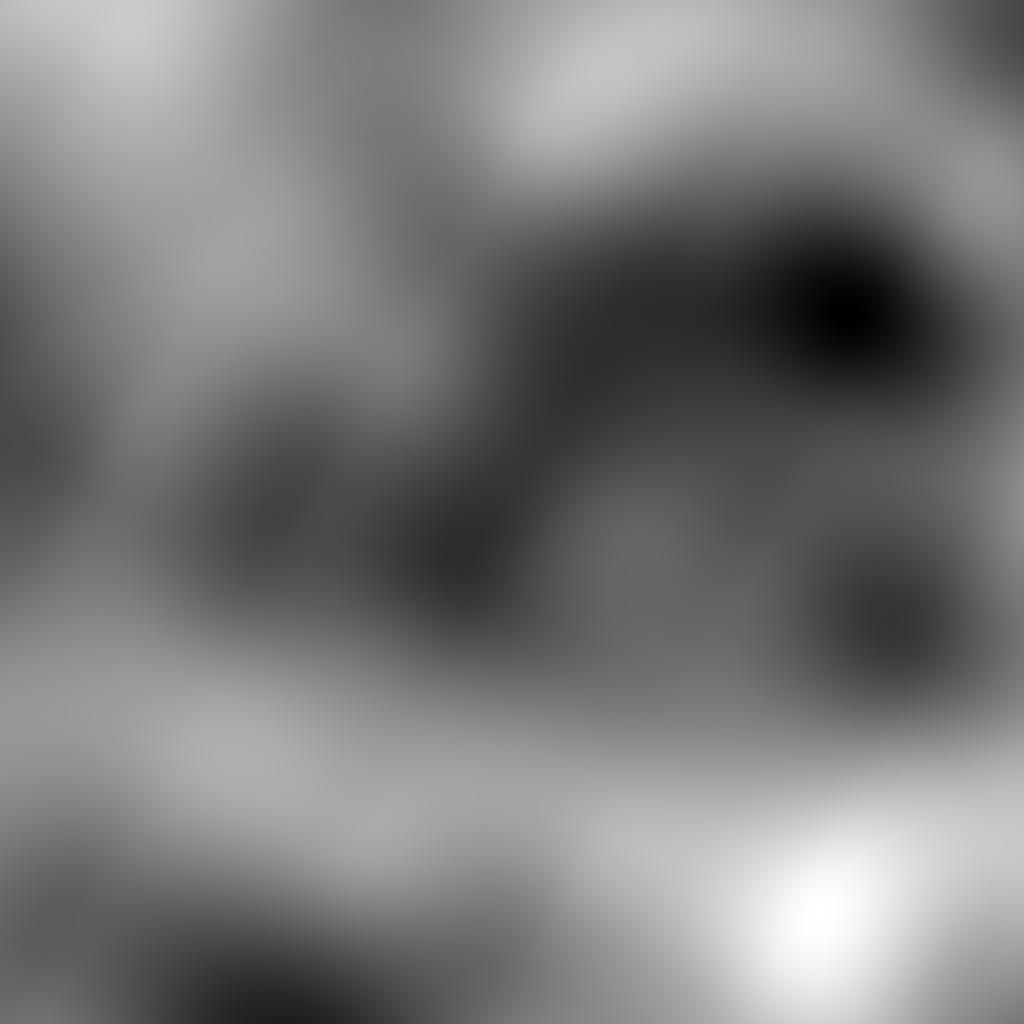
\includegraphics[width=0.4\textwidth]{out/simplefBm3/simplefBm3_gradval_noise3D_hermiteInterp_rot.png}
\caption{Simple brownian motion fractal with gradval noise 3D and hermite interpolation with rotation.}
\label{fig:simple_bm3_gradval_noise3D_hermiteInterp_rot}
\end{figure}

\begin{figure}[h]
\centering
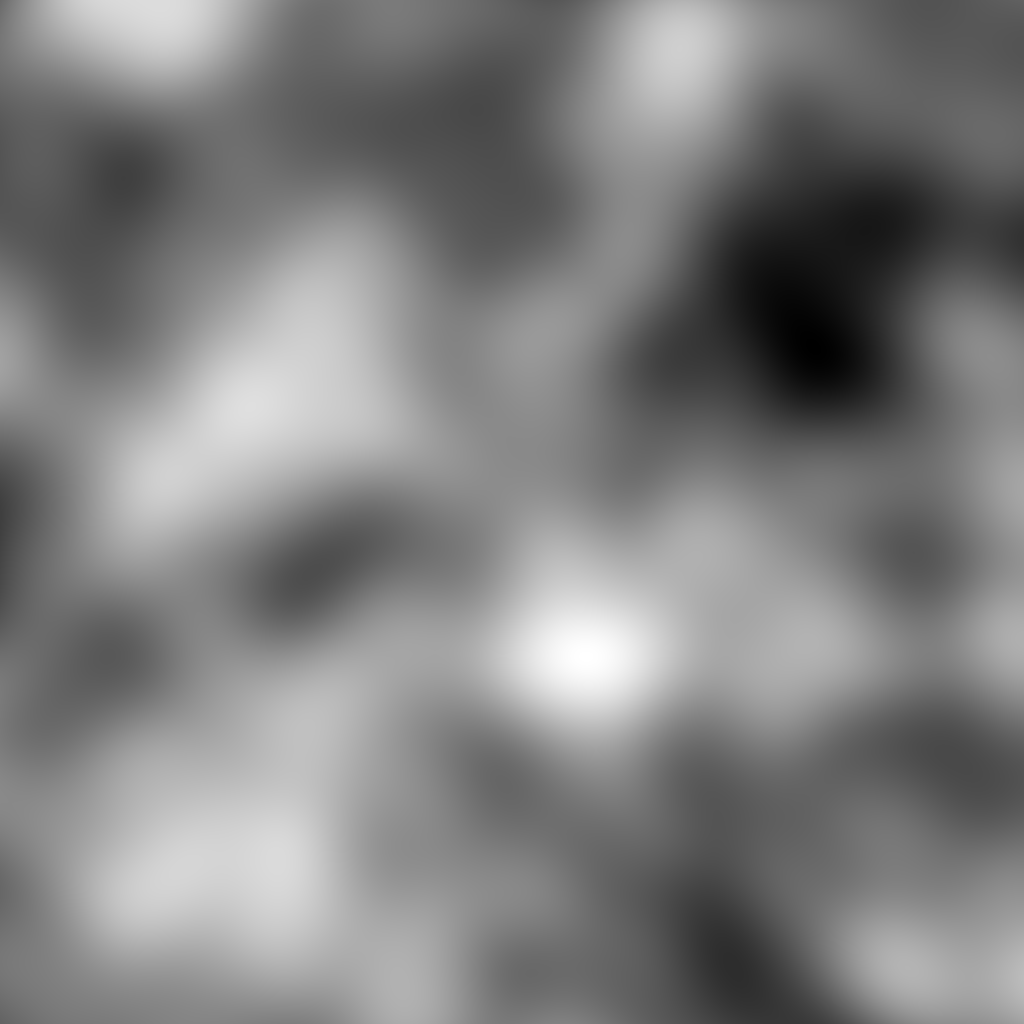
\includegraphics[width=0.4\textwidth]{out/simplefBm3/simplefBm3_simplex_noise3D_noInterp_rot.png}
\caption{Simple brownian motion fractal with simplex noise 3D with rotation.}
\label{fig:simple_bm3_simplex_noise3D_noInterp_rot}
\end{figure}

\index{simplefBm3}\index{simplefBm4}\index{simplefBm6}
\begin{lstlisting}[caption={Definition of simple brownian motion fractal functions},label={lst:simple_bm_fractal_definition},language=OpenCL]
simplefBm3(vector3 v, noise_func3 basistype, uint seed, interp_func interp, random_func rnd, void *srnd, uint numoctaves, REAL frequency, bool rot);
simplefBm4(vector4 v, noise_func4 basistype, uint seed, interp_func interp, random_func rnd, void *srnd, uint numoctaves, REAL frequency, bool rot);
simplefBm6(vector8 v, noise_func6 basistype, uint seed, interp_func interp, random_func rnd, void *srnd, uint numoctaves, REAL frequency, bool rot);
\end{lstlisting}

\begin{lstlisting}[caption={Example for simple brownian motion fractal functions},label={lst:simple_bm_fractal_example},language=OpenCL]
kernel void map2d_image(
global struct SMappingRanges *g_ranges,
write_only image2d_t output
) {
    $insert_localMapRange
    long seed = 200;
    kiss09_state srnd;
    kiss09_seed(&srnd, 200);
    // no rotation
    const float v = simplefBm3(coord[i], value_noise3D, 200, noInterp, random_kiss09, &srnd, 3, 0.125, false);
    // with rotation
    const float v = simplefBm3(coord[i], value_noise3D, 200, noInterp, random_kiss09, &srnd, 3, 0.125, true);
    write_imagef(output, (int2)(g0, g1), (float4)(v, v, v, 1.0));
}
\end{lstlisting}

Returns fractional brownian motion value for the coordinate.

\begin{figure}[h]
\centering
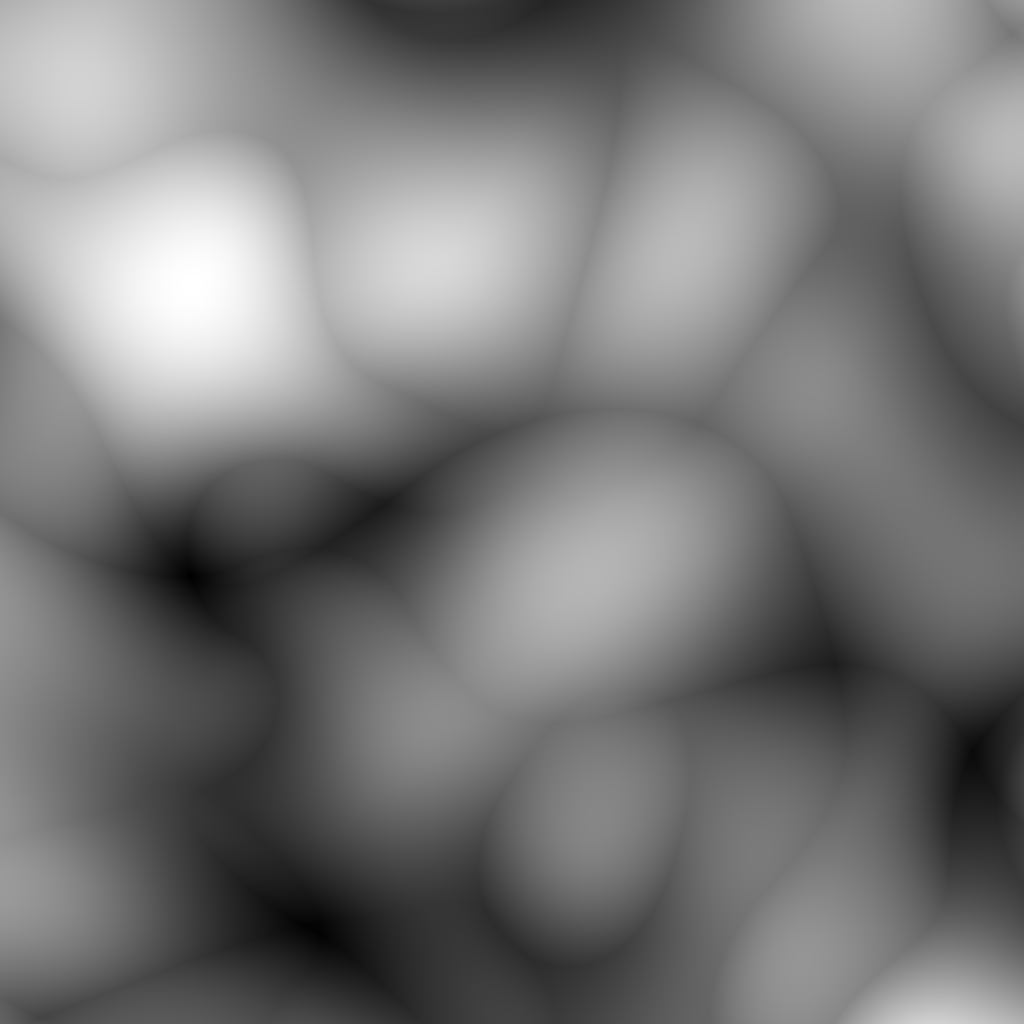
\includegraphics[width=0.4\textwidth]{out/simpleRidgedMultifractal3/simpleRidgedMultifractal3_value_noise3D_hermiteInterp_rot.png}
\caption{Simple ridged-multifractal with value noise 3D and hermite interpolation with rotation.}
\label{fig:simple_redgedmf3_value_noise3D_hermiteInterp_rot}
\end{figure}

\begin{figure}[h]
\centering
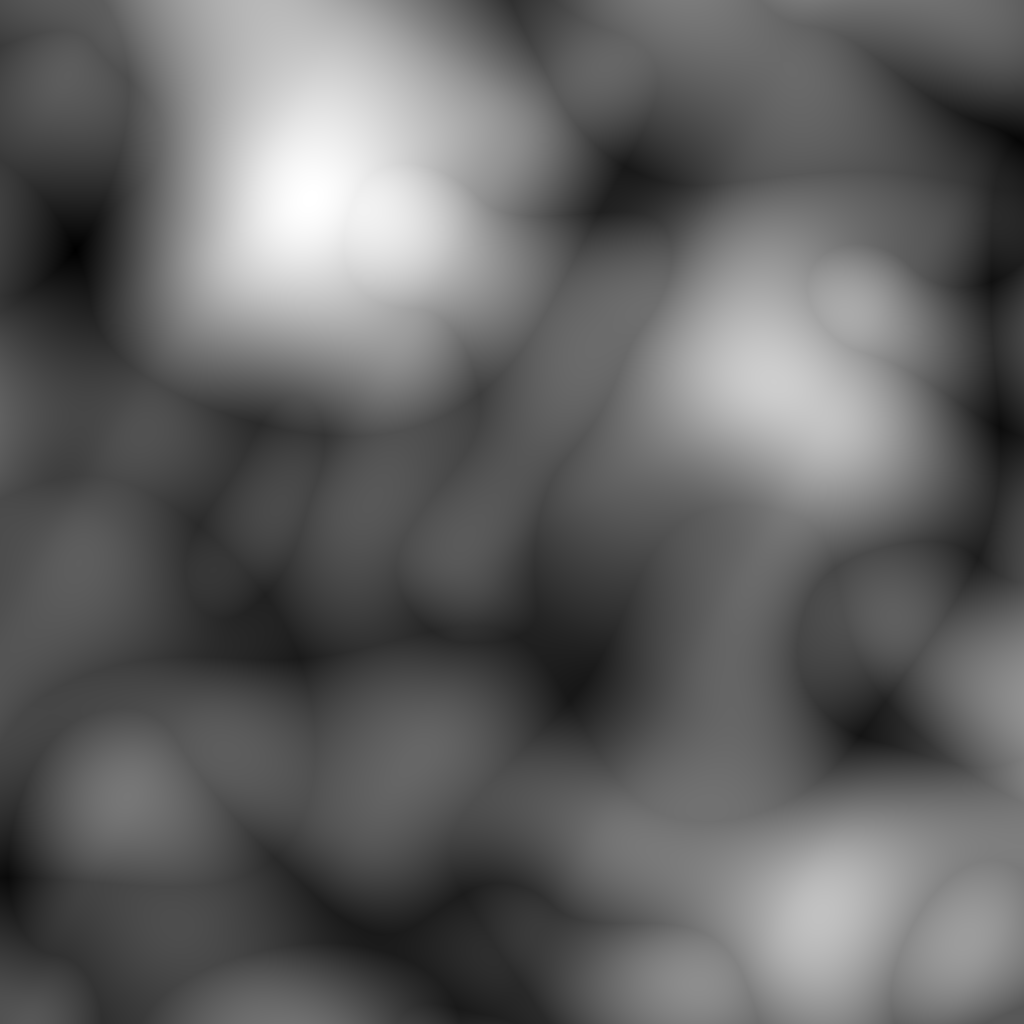
\includegraphics[width=0.4\textwidth]{out/simpleRidgedMultifractal3/simpleRidgedMultifractal3_gradient_noise3D_hermiteInterp_rot.png}
\caption{Simple ridged-multifractal with gradient noise 3D and linear hermite with rotation.}
\label{fig:simple_redgedmf3_gradient_noise3D_hermiteInterp_rot}
\end{figure}

\begin{figure}[h]
\centering
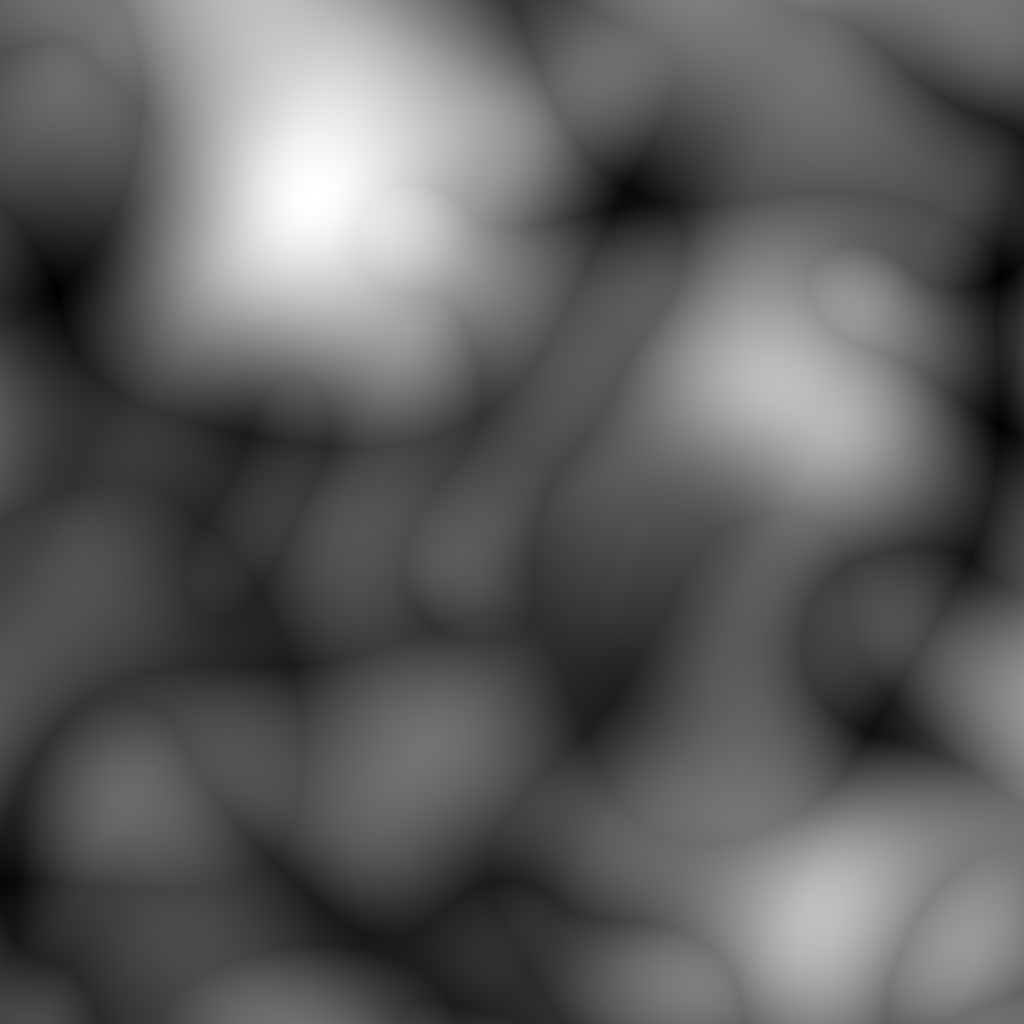
\includegraphics[width=0.4\textwidth]{out/simpleRidgedMultifractal3/simpleRidgedMultifractal3_gradval_noise3D_hermiteInterp_rot.png}
\caption{Simple ridged-multifractal with gradval noise 3D and hermite interpolation with rotation.}
\label{fig:simple_redgedmf3_gradval_noise3D_hermiteInterp_rot}
\end{figure}

\begin{figure}[h]
\centering
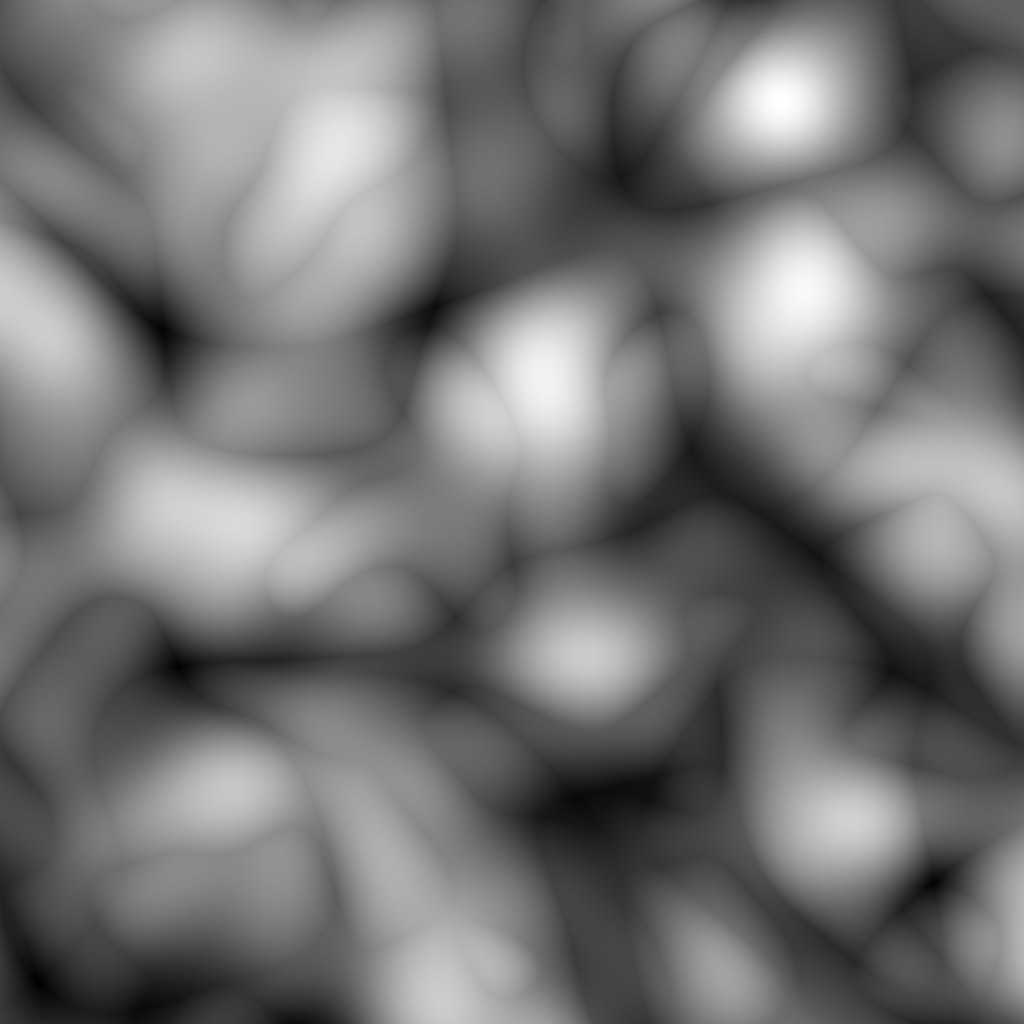
\includegraphics[width=0.4\textwidth]{out/simpleRidgedMultifractal3/simpleRidgedMultifractal3_simplex_noise3D_noInterp_rot.png}
\caption{Simple ridged-multifractal with simplex noise 3D with rotation.}
\label{fig:simple_redgedmf3_simplex_noise3D_noInterp_rot}
\end{figure}

\index{simplefBm3}\index{simplefBm4}\index{simplefBm6}
\begin{lstlisting}[caption={Definition of simple ridged multi-fractal functions},label={lst:simple_redgedmf3_definition},language=OpenCL]
simpleRidgedMultifractal3(vector3 v, noise_func3 basistype, uint seed, interp_func interp, random_func rnd, void *srnd, uint numoctaves, REAL frequency, bool rot);
simpleRidgedMultifractal4(vector4 v, noise_func4 basistype, uint seed, interp_func interp, random_func rnd, void *srnd, uint numoctaves, REAL frequency, bool rot);
simpleRidgedMultifractal6(vector8 v, noise_func6 basistype, uint seed, interp_func interp, random_func rnd, void *srnd, uint numoctaves, REAL frequency, bool rot);
\end{lstlisting}

\begin{lstlisting}[caption={Example for simple ridged multi-fractal functions},label={lst:simple_redgedmf3_example},language=OpenCL]
kernel void map2d_image(
global struct SMappingRanges *g_ranges,
write_only image2d_t output
) {
    $insert_localMapRange
    long seed = 200;
    kiss09_state srnd;
    kiss09_seed(&srnd, 200);
    // no rotation
    const float v = simpleRidgedMultifractal3(coord[i], value_noise3D, 200, noInterp, random_kiss09, &srnd, 3, 0.125, false);
    // with rotation
    const float v = simpleRidgedMultifractal3(coord[i], value_noise3D, 200, noInterp, random_kiss09, &srnd, 3, 0.125, true);
    write_imagef(output, (int2)(g0, g1), (float4)(v, v, v, 1.0));
}
\end{lstlisting}

Returns ridged-multifractal noise value for the coordinate.

\begin{figure}[h]
\centering
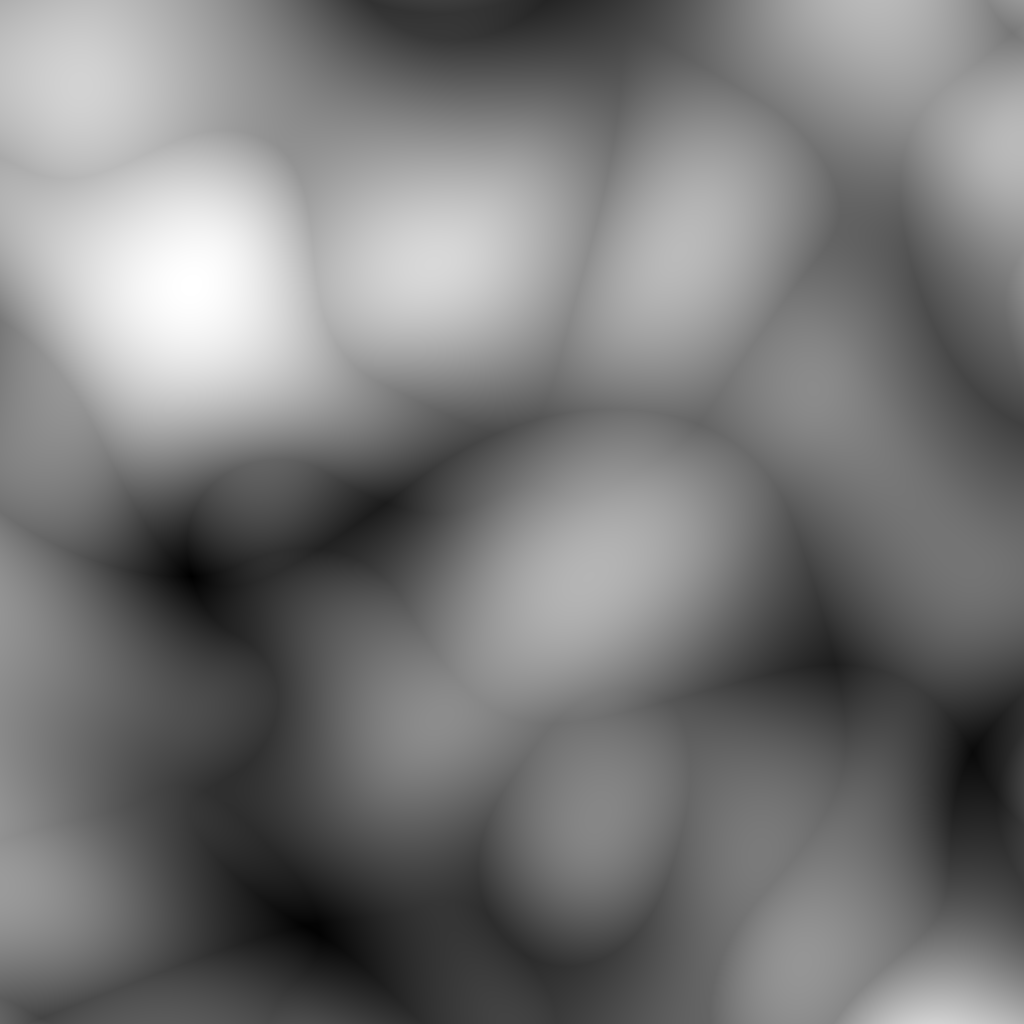
\includegraphics[width=0.4\textwidth]{out/simpleBillow3/simpleBillow3_value_noise3D_hermiteInterp_rot.png}
\caption{Simple billow fractal with value noise 3D and hermite interpolation with rotation.}
\label{fig:simple_billow3_value_noise3D_hermiteInterp_rot}
\end{figure}

\begin{figure}[h]
\centering
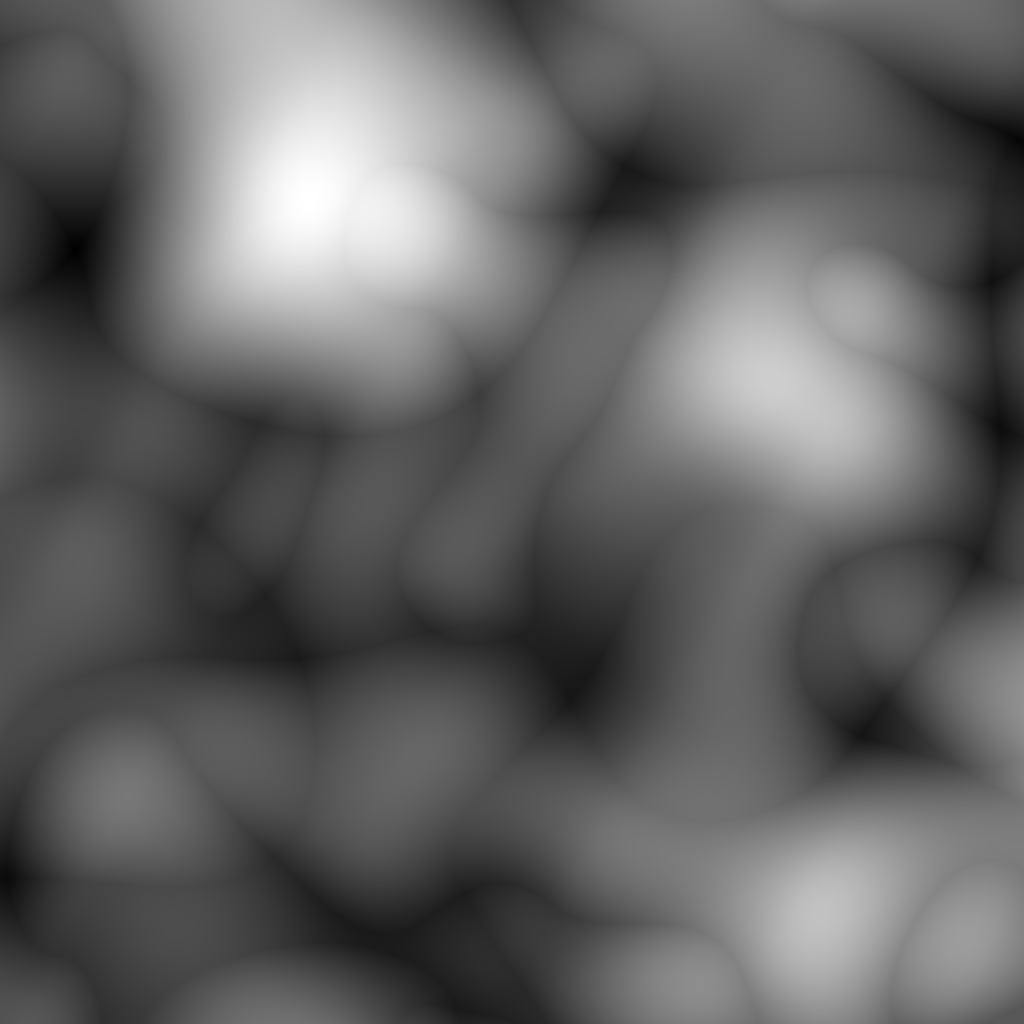
\includegraphics[width=0.4\textwidth]{out/simpleBillow3/simpleBillow3_gradient_noise3D_hermiteInterp_rot.png}
\caption{Simple billow fractal with gradient noise 3D and linear hermite with rotation.}
\label{fig:simple_billow3_gradient_noise3D_hermiteInterp_rot}
\end{figure}

\begin{figure}[h]
\centering
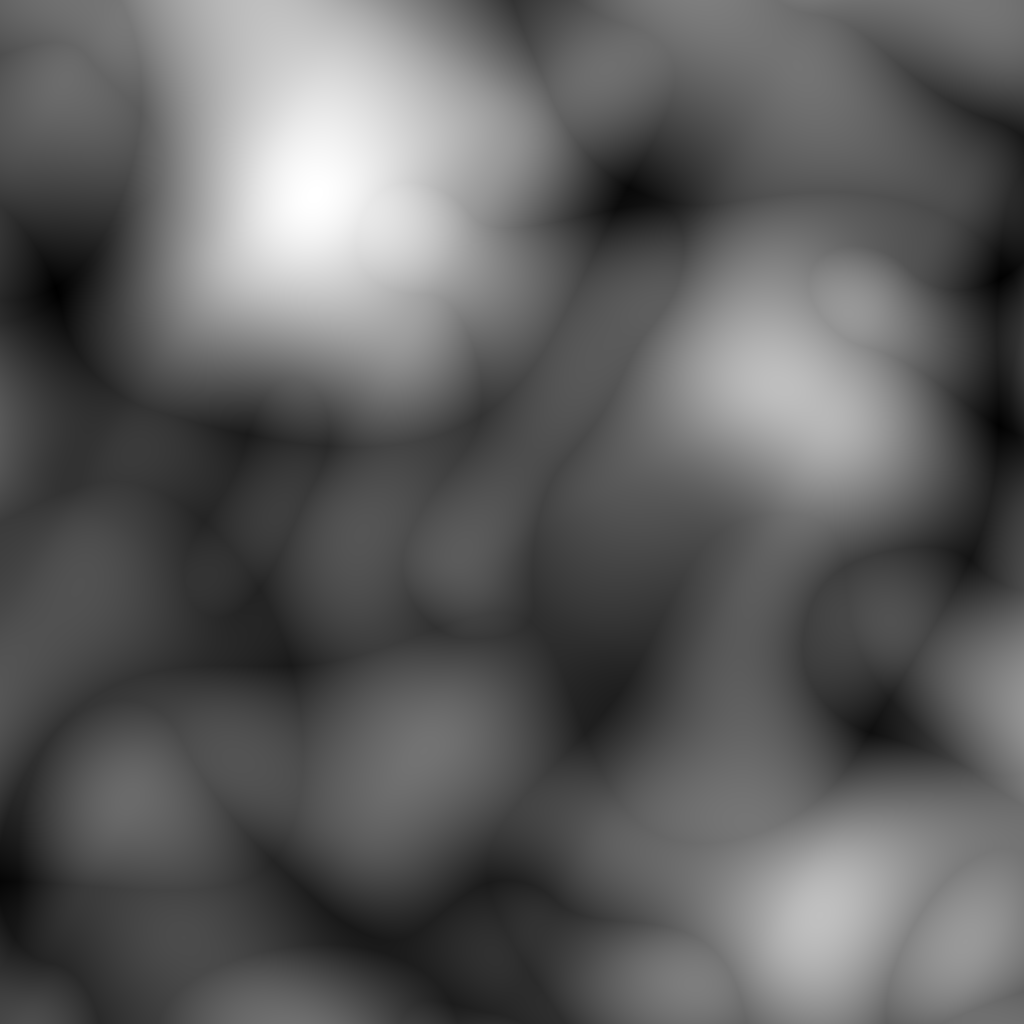
\includegraphics[width=0.4\textwidth]{out/simpleBillow3/simpleBillow3_gradval_noise3D_hermiteInterp_rot.png}
\caption{Simple billow fractal with gradval noise 3D and hermite interpolation with rotation.}
\label{fig:simple_billow3_gradval_noise3D_hermiteInterp_rot}
\end{figure}

\begin{figure}[h]
\centering
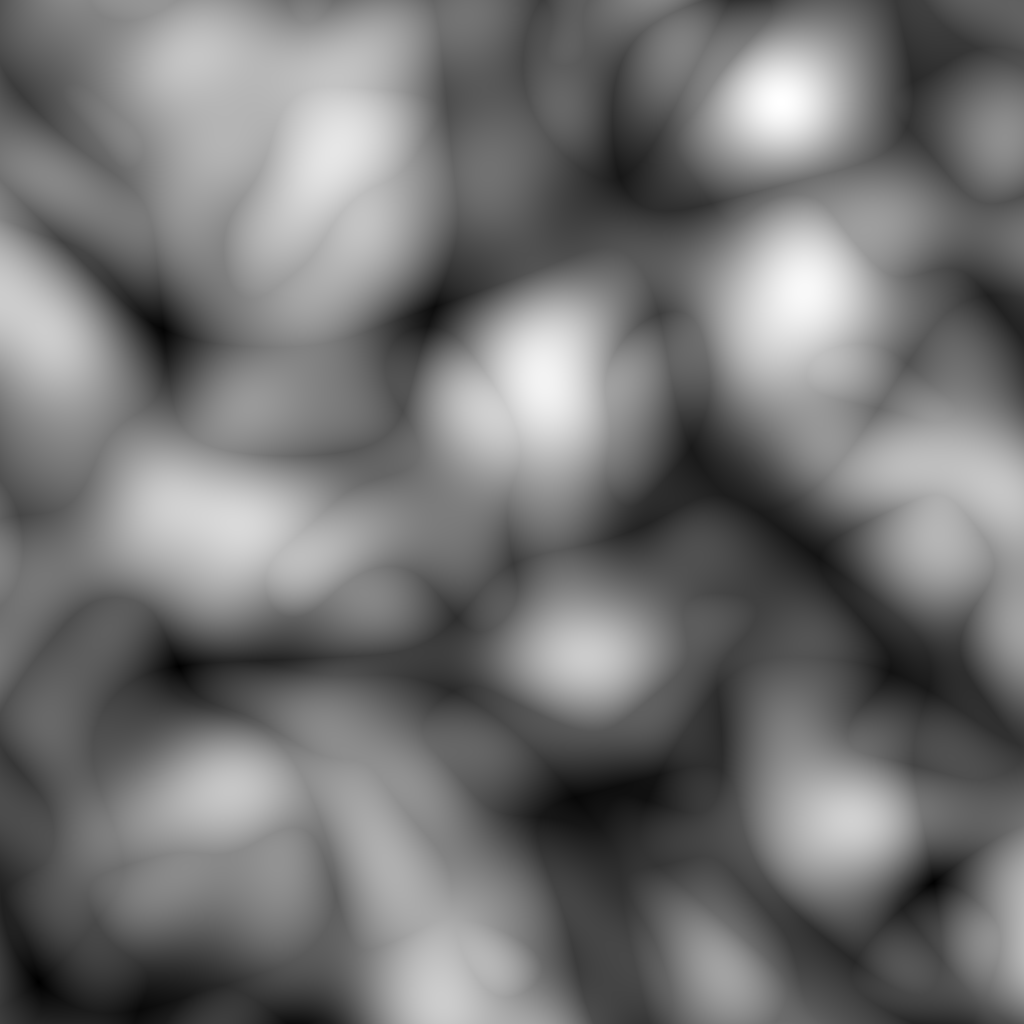
\includegraphics[width=0.4\textwidth]{out/simpleBillow3/simpleBillow3_simplex_noise3D_noInterp_rot.png}
\caption{Simple billow fractal with simplex noise 3D with rotation.}
\label{fig:simple_billow3_simplex_noise3D_noInterp_rot}
\end{figure}

\index{simpleBillow3}\index{simpleBillow4}\index{simpleBillow6}
\begin{lstlisting}[caption={Definition of simple billow fractal functions},label={lst:simple_billow_definition},language=OpenCL]
simpleBillow3(vector3 v, noise_func3 basistype, uint seed, interp_func interp, random_func rnd, void *srnd, uint numoctaves, REAL frequency, bool rot);
simpleBillow4(vector4 v, noise_func4 basistype, uint seed, interp_func interp, random_func rnd, void *srnd, uint numoctaves, REAL frequency, bool rot);
simpleBillow6(vector8 v, noise_func6 basistype, uint seed, interp_func interp, random_func rnd, void *srnd, uint numoctaves, REAL frequency, bool rot);
\end{lstlisting}

\begin{lstlisting}[caption={Example for simple billow fractal functions},label={lst:simple_billow_example},language=OpenCL]
kernel void map2d_image(
global struct SMappingRanges *g_ranges,
write_only image2d_t output
) {
    $insert_localMapRange
    long seed = 200;
    kiss09_state srnd;
    kiss09_seed(&srnd, 200);
    // no rotation
    const float v = simpleBillow3(coord[i], value_noise3D, 200, noInterp, random_kiss09, &srnd, 3, 0.125, false);
    // with rotation
    const float v = simpleBillow3(coord[i], value_noise3D, 200, noInterp, random_kiss09, &srnd, 3, 0.125, true);
    write_imagef(output, (int2)(g0, g1), (float4)(v, v, v, 1.0));
}
\end{lstlisting}

Returns billow (cloud-like, lumpy) fractal value for the coordinate.

\subsubsection{Other Functions}

\index{x}\index{y}\index{z}\index{w}\index{u}\index{v}
\begin{lstlisting}[caption={Definition of components functions},label={lst:components_definition},language=OpenCL]
x(v)
y(v)
z(v)
w(v)
u(v)
v(v)
\end{lstlisting}

\begin{lstlisting}[caption={Example for components functions},label={lst:components_example},language=OpenCL]
kernel void map2d_image(
global struct SMappingRanges *g_ranges,
write_only image2d_t output
) {
    $insert_localMapRange
    const float x = x(coord[i]);
    const float y = y(coord[i]);
    const float z = z(coord[i]);
    const float w = w(coord[i]);
    const float u = u(coord[i]);
    const float v = v(coord[i]);
}
\end{lstlisting}

Returns the x, y, z, w, u and v component of the vector.

\index{random\_func}
\begin{lstlisting}[caption={Definition of random function type},label={lst:random_type_definition},language=OpenCL]
typedef REAL (*random_func)(void*);
\end{lstlisting}

Function that returns a random number.
